\documentclass{article}
\usepackage{amsmath}
\usepackage{amssymb}
\usepackage{graphicx}
\graphicspath{ {./images/} }

\title{Mathematics for Computer Science Summative - Elis Mostyn}
\begin{document}
	\maketitle
	\newpage
	\section {Discrete Mathematics and Linear Algrebra}
	\subsection*{1}
	$ 2^{n+5} \cdot 3^{4n} + 5^{3n+1} = 37m$
	\newline
	Base Case:  n =1 
	\newline
	$ 2^6 \cdot 3^4 + 5^4 = 37m$
	\newline
	$64\cdot81 + 625 = 37m$
	\newline
	$5184 + 625 = 37m$
	\newline
	$5809 = 37m$
	\newline
	So for n=1, m = 157. Hence n = 1 holds
	\newline
	Assume that n = k holds, where:
	\newline
	$ 2^{k+5} \cdot 3^{4k} + 5^{3k+1} = 37m $
	\newline
	\newline
	Let n = k+ 1 $ = 2^{k+6} \cdot 3^{4k+4} + 5^{3k+4}  $
	\newline
	$ 124 \cdot (2^{k+5} \cdot 3^{4k} + 5^{3k+1})+37\cdot(2^{k+5} \cdot 3^{4k}\cdot161)=37c$
	\newline
	$2^{k+5} \cdot 3^{4k}\cdot161 + 5^{3k+1}\cdot124 = 37c$
	\newline
	$2^{k+5}\cdot3^{4k}(2\cdot3^4-1)+ 5^{3k+1}(5^3-1)=37c$
	\newline
	$(2^{k+6}\cdot3^{4k+4}-2^{k+5}\cdot3^{4k}) +(5^{3k+4}-5^{3k+1}) = 37c $
	\newline
	$(2^{k+6}\cdot3^{4k+4}+5^{3k+4})-(2^{k+5}\cdot3^{4k}+5^{3k+1}) = 37c $
	\newline
	$2^{k+6}\cdot3^{4k+4}+5^{3k+4} = 37m$
	\newline
	As n=k+1 holds we can say that:
	\newline
	$ 2^{n+5} \cdot 3^{4n} + 5^{3n+1}  $
	\newline
	Is divisible by 37 for all $ n \geqslant 1 $

	\subsection*{2}
	To visualise the number of bit strings, we  will first provide example numbers.
	\newline
	Let $ n=30$ so there are 30 '0s'
	\newline
	Let $ k=4$ so there are 4 '1s'
	\newline
	No restrictions on position of 1s: $\binom{34}{4}$
	\newline
	At least one zero between each 1 (m=1) so 1s look like:
	\newline
	10 10 10 1 
	\newline
	Taking each of the above as an indivdual item, there are 27 other '0s'  and 4 groups of '1s'. Hence the combinations are: $\binom{31}{4}$
	\newline
	At least two zeroes between each 1 (m=2) so 1s look like:
	\newline
	100 100 100 1
	\newline
	Again, taking each of the above as an individual item, there are 24 other '0s' and once again 4 groups of '1s'. So the combinations are: $\binom{28}{4}$
	\newline
	\newline
	Using this example we can see a pattern occuring: where the number of combinations of bit strings is:
	\newline
	\begin{center}
	$\binom{NumOf0s + NumOf1s - NumBetween(NumOf1s -1)}{NumOf1s}$
	\end{center}
	Which in terms of n,k and m is:
	\newline
	\begin{center}
	$\binom{n+k-m\cdot(k-1)}{k}$
	\end{center}
	\subsection*{3}
	To identify the probability that neither of the outcomes appears 3 times in a row, we will first identify the probability of that occuring. 
	\newline
	Each of the  $2^{10}$ outcomes can be viewed as a bit string.
	\newline
	Then using a program in python we can see where three of the same outcome occurs:
	\newline
	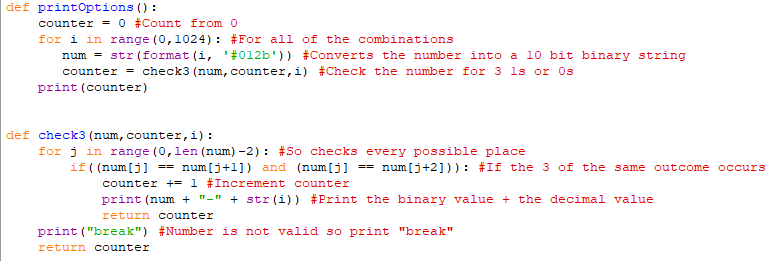
\includegraphics[width=\textwidth]{Pycode}
	\newline
	Starting at 0000000000, we can count the ranges in which it occurs:
	\begin{center}
	\begin{tabular}{|c|c|c|}
	\hline
	Begin & End & Number of Combinations\\
	\hline
	0000000000&0010010001&146 \\
	\hline
	0010010111&0010011000&2 \\
	\hline
	0010011100&0010100011&8\\
	\hline
	0010100111&0010101000&2\\
	\hline
	0010101110&0010110001&4\\
	\hline
	0010110111&0011001000&18\\
	\hline
	0011001110&0011010001&4\\
	\hline
	0011010111&0011011000&2\\
	\hline
	0011011100&0100100011&72\\
	\hline
	0100100111&0100101000&2\\
	\hline
	0100101110&0100110001&4\\
	\hline
	0100110111&0101001000&18\\
	\hline
	0101001110&0101010001&4\\
	\hline
	0101010111&0101011000&2\\
	\hline
	0101011100&0101100011&8\\
	\hline
	0101100111&0101101000&2\\
	\hline
	0101101110&0110010001&36\\
	\hline
	0110010111&0110011000&2\\
	\hline
	0110011100&0110100011&8\\
	\hline
	0110100111&0110101000&2\\
	\hline
	0110101110&0110110001&4\\
	\hline
	0110110111&1001001000&146\\
	\hline
	1001001110&1001010001&4\\
	\hline
	1001010111&1001011000&2\\
	\hline
	1001011100&1001100011&8\\
	\hline
	1001100111&1001101000&2\\
	\hline
	1001101110&1010010001&36\\
	\hline
	1010010111&1010011000&2\\
	\hline
	1010011100&1010100011&8\\
	\hline
	1010100111&1010101000&2\\
	\hline
	1010101110&1010110001&4\\
	\hline
	1010110111&1011001000&18\\
	\hline
	1011001110&1011010001&4\\
	\hline
	1011010111&1011011000&2\\
	\hline
	1011011100&1100100011&72\\
	\hline
	1100100111&1100101000&2\\
	\hline
	1100101110&1100110001&4\\
	\hline
	1100110111&1101001000&18\\
	\hline
	1101001110&1101010001&4\\
	\hline
	1101010111&1101011000&2\\
	\hline
	1101101110&1111111111&146\\
	\hline
	\end{tabular}
	\end{center}
	Total = 846 Combinations where 3 of either outcomes occurs.
	\newline
	P(No outcome 3 times in a row) = 1 - $\frac{846}{1024}$
	\newline
	P(No outcome 3 times in a row) =$\frac{89}{512}$
	
	\subsection*{4}
	If variable X is equal to the number of the umbrellas left on the bus. Then:
	\newline
	ExpectedValue(X) =$4\cdot P(all 4 left) + 3\cdot P(exactly 3 left) + 2\cdot P(exactly 2 left) + 1 \cdot P(exactly 1 left) + 0\cdot P(none left) $
	\newline
	P(all 4 left) = ($0.4\cdot0.5\cdot0.6\cdot0.8$)
	\newline
	P(all 4 left) = $0.096$
	\newline
	P(Exactly 3 Left):
	\begin{center}
	\begin{tabular}{|c|c|}
	\hline
	Combination&Probability\\
	\hline
	P1,P2,P3,$\neg$ P4&0.024 \\	
	\hline
	P1,P2,P4,$\neg$ P0&0.064 \\
	\hline
	P1,P3,P4,$\neg$P2 & 0.096\\
	\hline
	P2,P3,P4,$\neg$P1&0.144 \\
	\hline
	Total & 0.328\\
	\hline
	\end{tabular}
	\end{center}
	P(Exactly 2 Left):
	\begin{center}
	\begin{tabular}{|c|c|}
	\hline
	Combination&Probability\\
	\hline
	P1,P2,$\neg$P3,$\neg$P4&0.016\\
	\hline
	P1,$\neg$P2,P3,$\neg$P4&0.024\\
	\hline
	P1,$\neg$P2,$\neg$P3,P4&0.064\\
	\hline
	$\neg$P1,P2,P3,$\neg$P4&0.036\\
	\hline
	$\neg$P1,P2,$\neg$P3,P4&0.096\\
	\hline
	$\neg$P1,$\neg$P2,P3,P4&0.144\\
	\hline
	Total & 0.364\\
	\hline
	\end{tabular}
	\end{center}
	P(Exactly 1 Left)
	\begin{center}
	\begin{tabular}{|c|c|}
	\hline
	Combination&Probability\\
	\hline
	P1,$\neg$P2,$\neg$P3,$\neg$P4&0.016\\
	\hline
	$\neg$P1,P2,$\neg$P3,$\neg$P4&0.024\\
	\hline
	$\neg$P1,$\neg$P2,P3,$\neg$P4&0.036\\
	\hline
	$\neg$P1,$\neg$P2,$\neg$P3,P4&0.096\\
	\hline
	Total&0.172\\
	\hline
	\end{tabular}
	\end{center}	
	P(None left) = $0.6\cdot0.5\cdot0.4\cdot0.2$
	\newline
	P(None left) = 0.024
	\newline
	\newline
	Expected Value = $4(0.096)+3(0.328)+2(0.364)+1(0.172)+0(0.024)$
	\newline
	Expected Value = $0.384+0.984+0.728+0.172+0$
	\newline
	Expected Value = $2.268$
	\newline
	\newline
	Variance(x) = E($x^2$) - (E(x))$^2$
	\newline
	Variance(x) =$ 16\cdot(0.096) + 9\cdot(0.328) + 4\cdot(0.364) + 1\cdot(0.172) + 0\cdot(0.024) - (2.0268)^2$
	\newline
	Variance(x) = $6.116-(2.268)^2$
	\newline
	Variance(x) = $0.972$

	\subsection*{5}
	For n=4, there exists a graph with diameter 2:
	\newline
	With k = 1
	\newline
	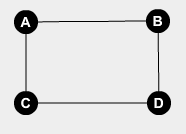
\includegraphics{4None2}
	\newline
	Where the cycle is as follows:
	\newline
	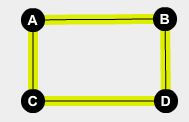
\includegraphics{41Cycle1}
	\newline
	With k =3
	\newline
	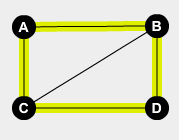
\includegraphics{43Cycles1}
	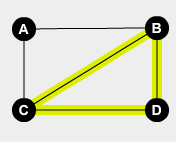
\includegraphics{43Cycles2}
	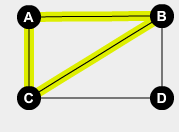
\includegraphics{43Cycles3}
	\newline
	k=0 Doesn't exist for diameter 2 as removing an edge makes the diameter 3.
	\newline
	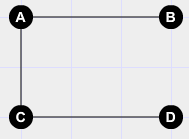
\includegraphics{40None}
	\newline
	For n = 5, there exists a graph with diameter 3
	\newline
	With k =1
	\newline
	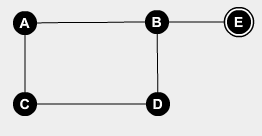
\includegraphics{5None1}
	\newline
	Where the cycle is as follows
	\newline
	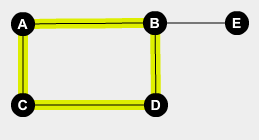
\includegraphics{51Cycle1}
	\newline
	With k=3
	\newline
	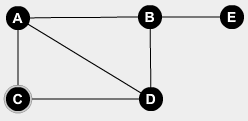
\includegraphics{5None2}
	\newline
	With cycles as follows:
	\newline
	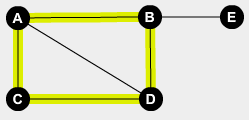
\includegraphics{53Cycle1}
	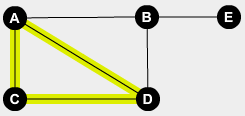
\includegraphics{53Cycle2}
	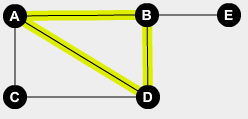
\includegraphics{53Cycle3}
	\newline
	For any n$\geq$4 a graph can be drawn which has a diameter of n-2 and k=1 and k=3 by adding an extra vertex in a chain from "B".
	\newline
	And either having an edge between A \& D for k=3 or not for k=1
	\newline
	k=2 cannot exist in a graph because adding another edge to a graph where k=1 holds will add an extra 2 cycles.
	For example n = 6:
	\newline
	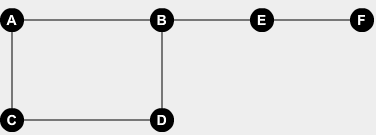
\includegraphics{6None}
	\newline
	Which holds for k=1
	\newline
	No edge can be added which adds only 1 cycle, even ignoring the n-2 diameter requirement:
	\newline
	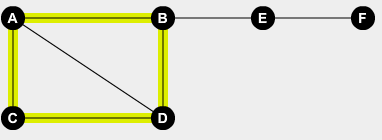
\includegraphics{6Cycles1}
	\newline
	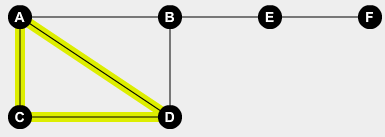
\includegraphics{6Cycles2}
	\newline
	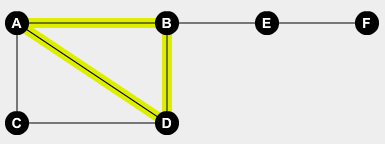
\includegraphics{6Cycles3}
	\newline
	\newline
	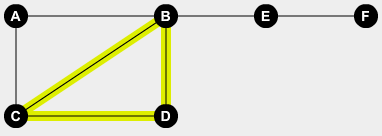
\includegraphics{6Cycles4}
	\newline
	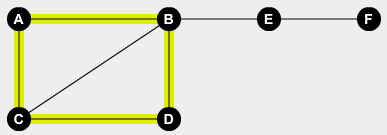
\includegraphics{6Cycles5}
	\newline
	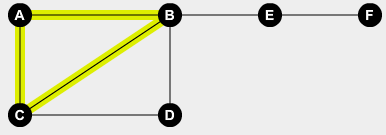
\includegraphics{6Cycles6}
	\newline
	\newline
	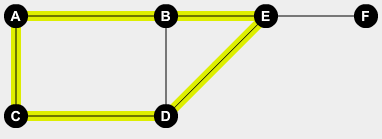
\includegraphics{6Cycles7}
	\newline
	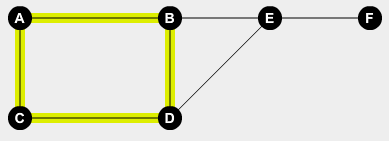
\includegraphics{6Cycles8}
	\newline
	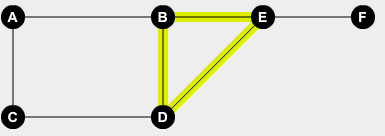
\includegraphics{6Cycles9}
	\newline
	\newline
	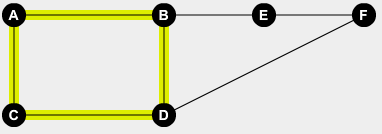
\includegraphics{6Cycles10}
	\newline
	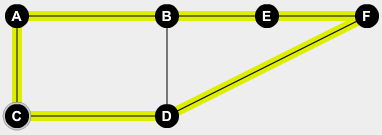
\includegraphics{6Cycles11}
	\newline
	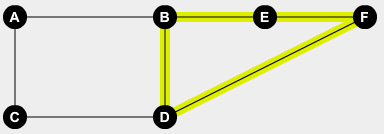
\includegraphics{6Cycles12}
	\newline
	Therefore $k \neq 2$
	\newline
	Furthermore, for n-2 diameter, $ 1 \geq k \leq 3$ as adding more edges to increase cycles will decrease the diameter.

	\section{Logic and Discrete Structures}
	\subsection*{6a}
	To convert a formula to disjunctive normal form using truth tables, 
	\begin{center}
	\begin{tabular}{ |c|c|c|c|c|c| } 
 	\hline
 	 $ a $ & $ b$ & $c$ & $ \neg a\land \neg b $ & $( a \land b) \implies c $ & $\neg( a\land b \implies c )\lor \neg a \land \neg b $ \\ 
	\hline
	0&0&0&1&1&1 \\
	\hline
	0&0&1&1&1&1\\
	\hline
	0&1&0&0&1&0 \\
	\hline
	0&1&1&0&1&0 \\
	\hline
	1&0&0&0&1&0 \\
	\hline
	1&0&1&0&1&0 \\
	\hline
	1&1&0&0&0&1 \\
	\hline
	1&1&1&0&1&0 \\
	\hline
	\end{tabular}
	\end{center}
	
	$\varphi = (\neg a \land \neg b \land \neg c)  \lor (\neg a \land \neg b \land c) \lor (a \land b \land \neg c)$
	\newline
	Although, due to $\neg c \lor c $
	\newline
	$\varphi = (\neg a \land \neg b) \lor (a \land b \land \neg c)$

	\subsection*{6b.}
	$ \neg \varphi = \neg( (\neg a \land \neg b) \lor (a \land b \land \neg c))$
	\newline
	$\neg \varphi = (a \lor b) \land (\neg a \lor \neg b \lor c)$
	
	\subsection*{7}
	To prove a set functionally complete we must prove it can represent all the logical operators of the set:
	\newline
	$\{\lor,\land,\neg\}$
	\newline
	As that is a set we know to be functionally complete:
	\newline
	If $P \bowtie Q \equiv (P \iff Q) \lor P$
	\newline 
	Then the truth table is as follows
	\begin{center}
	\begin{tabular}{|c|c|c|c|}
	\hline
	$P$ & $Q$ & $P\iff Q$ & $ (P \iff Q) \land P$\\
	\hline
	0&0&1&0\\
	\hline
	0&1&0&0\\
	\hline
	1&0&0&0\\
	\hline
	1&1&1&1\\
	\hline
	\end{tabular}
	\end{center}
	From this truth table we can see that $P \bowtie Q \equiv P \land Q$
	\newline
	As a result we can say that the logical operator $\land$ can be produced from the set $  \{\lor,\bowtie\}$
	\newline
	Providing truth premises to the set produces this:
	\newline
	\begin{center}
	\begin{tabular}{|c|c|c|c|}
	\hline
	P&Q&Operator&Output\\
	\hline
	1&1&$\lor$&1\\
	\hline
	1&1&$\bowtie$&1\\
	\hline
	\end{tabular}
	\end{center}
	This is significant because it means that the set is truth preserving. Meaning that it does not produce a false output given a true input. As a result of this, the set cannot represent the $\neg$ operator. 
	\newline
	Therefore, the set is not functionally complete.
	\subsection*{8a}
	1) $\neg (a \lor b) \land c$ \hspace{10mm}Premise
	\newline
	2) c  \hspace{25mm} $\land e (1)$
	\newline
	3) $ \neg (a \lor b) \hspace{16mm} \land e (1)$
	\newline
	4) \hspace{25mm}a \hspace{25mm} Assumption
	\newline
	5)\hspace{25mm} $ a \lor b \hspace{21mm} \lor i$
	\newline
	6) \hspace{25mm}$ \bot \hspace{27mm} \neg e (3,5)$
	\newline
	7)\hspace{25mm} $ b \hspace{27mm} Assumption$
	\newline
	8) \hspace{25mm}$ a \lor b \hspace{22mm} \lor i (7) $
	\newline
	9) \hspace{25mm}$ \bot \hspace{26mm} \neg e (3,8) $
	\newline
	10) $ \neg a \hspace{23mm} \neg i (4-6) $
	\newline 
	11) $ \neg b \hspace{23mm} \neg i (7-9) $
	\newline
	12) $ \neg b \land c \hspace{18mm} \land i (2,11)$
	\newline
	13) $ \neg a \land (\neg b \land c) \hspace{7 mm} \land i (10,12) $
	\newline
	\newline
	\newline

	\subsection*{8b}
	1)$ a \land b \hspace{27mm} Premise$
	\newline
	2) $ a \implies (\neg c \land \neg b) \hspace{7mm} Premise$
	\newline
	3)$ a \hspace{32mm} \land e (1) $
	\newline
	4) $ (\neg c \land \neg d) \hspace{14mm} \implies e (3),(2)$
	\newline
	5) $ \neg c \hspace{29mm} \land e (4) $
	\newline
	6) $ \neg d \hspace{29mm} \land e (4) $
	\newline
	7) \hspace{25mm}$ c \lor d \hspace{25mm} Assumption $
	\newline
	8)\hspace{25mm}$ \bot \hspace{29mm} \neg e (5),(6),(7) $
	\newline
	9) $ \neg ( c \lor d) \hspace{20mm} \neg i (7-8) $

	\subsection*{9}
	To identify whether $\varphi$ is a theorem, where:
	\newline
	$\varphi = \neg ((\neg t \lor \neg r) \land (p \lor p) \land (\neg p \lor \neg q) \land (r \lor p \lor q \lor \neg r) \land (t \lor s) 		\land (\neg r \lor \neg s \lor t) \land (q \lor r)) $
	\newline
	We must negate $\varphi$ to find $\neg \varphi$ and apply resolution continually until we have inferred the empty clause or reach a point where we cannot infer any new clauses.
	\newline
	\newline
	$\neg \varphi = ((\neg t \lor \neg r) \land (p \lor p) \land (\neg p \lor \neg q) \land (r \lor p \lor q \lor \neg r) \land (t \lor s) 		\land (\neg r \lor \neg s \lor t) \land (q \lor r)) $
	\newline
	\newline
	1) $ \neg t \lor \neg r $
	\newline
	2) $ p \lor p $
	\newline
	3) $ \neg p \lor \neg q $
	\newline
	4) $ r \lor p \lor q \lor \neg r $
	\newline
	5) $t \lor s$
	\newline
	6)$ \neg r \lor \neg s \lor t$
	\newline
	7)$ q \lor r $
	\newline
	8) $ \neg r \lor \neg s \hspace{15mm} Resolution - 1,6 $
	\newline
	9) $ \neg r \lor \neg t \hspace{15mm} Resolution -  5,8 $
	\newline
	10) $ t \lor \neg r \hspace{15.5mm} Resolution -  5,6 $
	\newline
	11) $ \neg r \lor \neg r\hspace{12.5mm} Resolution - 9,10 $
	\newline
	12) $ \neg r $
	\newline
	13) $ \neg q $\hspace{19.5mm} Resolution - 2,3
	\newline
	14) $ r $ \hspace{21mm} Resolution - 7,13
	\newline
	15) $ \phi $\hspace{21mm} 12,14
	\newline
	As $\neg \varphi$ Produces the empty clause, $\varphi$ must be always true, hence it is a theorem.
	
			`


\end{document}